\StartPlate{V27}{An odd-order action discrepancy can be summed away}{The correction acts on a supplied finite extension, not on an unconstructed arithmetic host.}
\begin{center}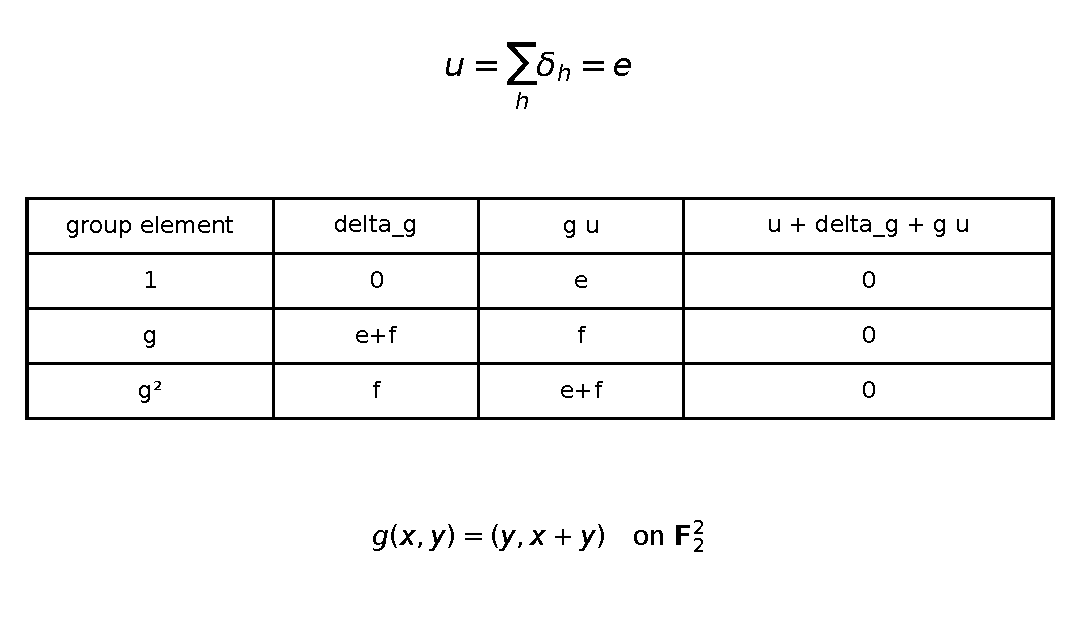
\includegraphics[width=\linewidth]{figures/V27.pdf}\end{center}
Let $C_3$ act on $A=\F_2^2$ by $g(x,y)=(y,x+y)$. Use the cocycle values $\delta_1=0$, $\delta_g=e+f$, and $\delta_{g^2}=f$. Their sum is $u=e$. The final column displays the corrected discrepancy, which is zero at every group element.
\[
\delta_{gh}=\delta_g+g\delta_h,
\qquad u=\sum_h\delta_h,
\qquad \delta_g=u+gu.
\]
The last identity follows by summing the cocycle equation and using that the group order is odd in characteristic two. Replacing the comparison by the vertical sign correction $u$ makes it equivariant.

In the extension theorem, the source and target already have genuine actions and an initial center-fixing extension isomorphism. The cocycle lives in the character space $\operatorname{Hom}(W,\F_2)$. The diagram is an exact module example of that calculation, not a new construction of those actions. A vertical correction may also be forbidden when particular lifts must remain unchanged.
\vfill\PlateSource{Exact C3-module model}{Part III, Section 29.1--29.2}{73}
